\subsection{Compact Objects \Contact{Simeon}}
\Contributors{Will D, Nathan G., Michael M., Simeon, George C.,...}
\label{sec:machos}

%\begin{figure}
%\centering
%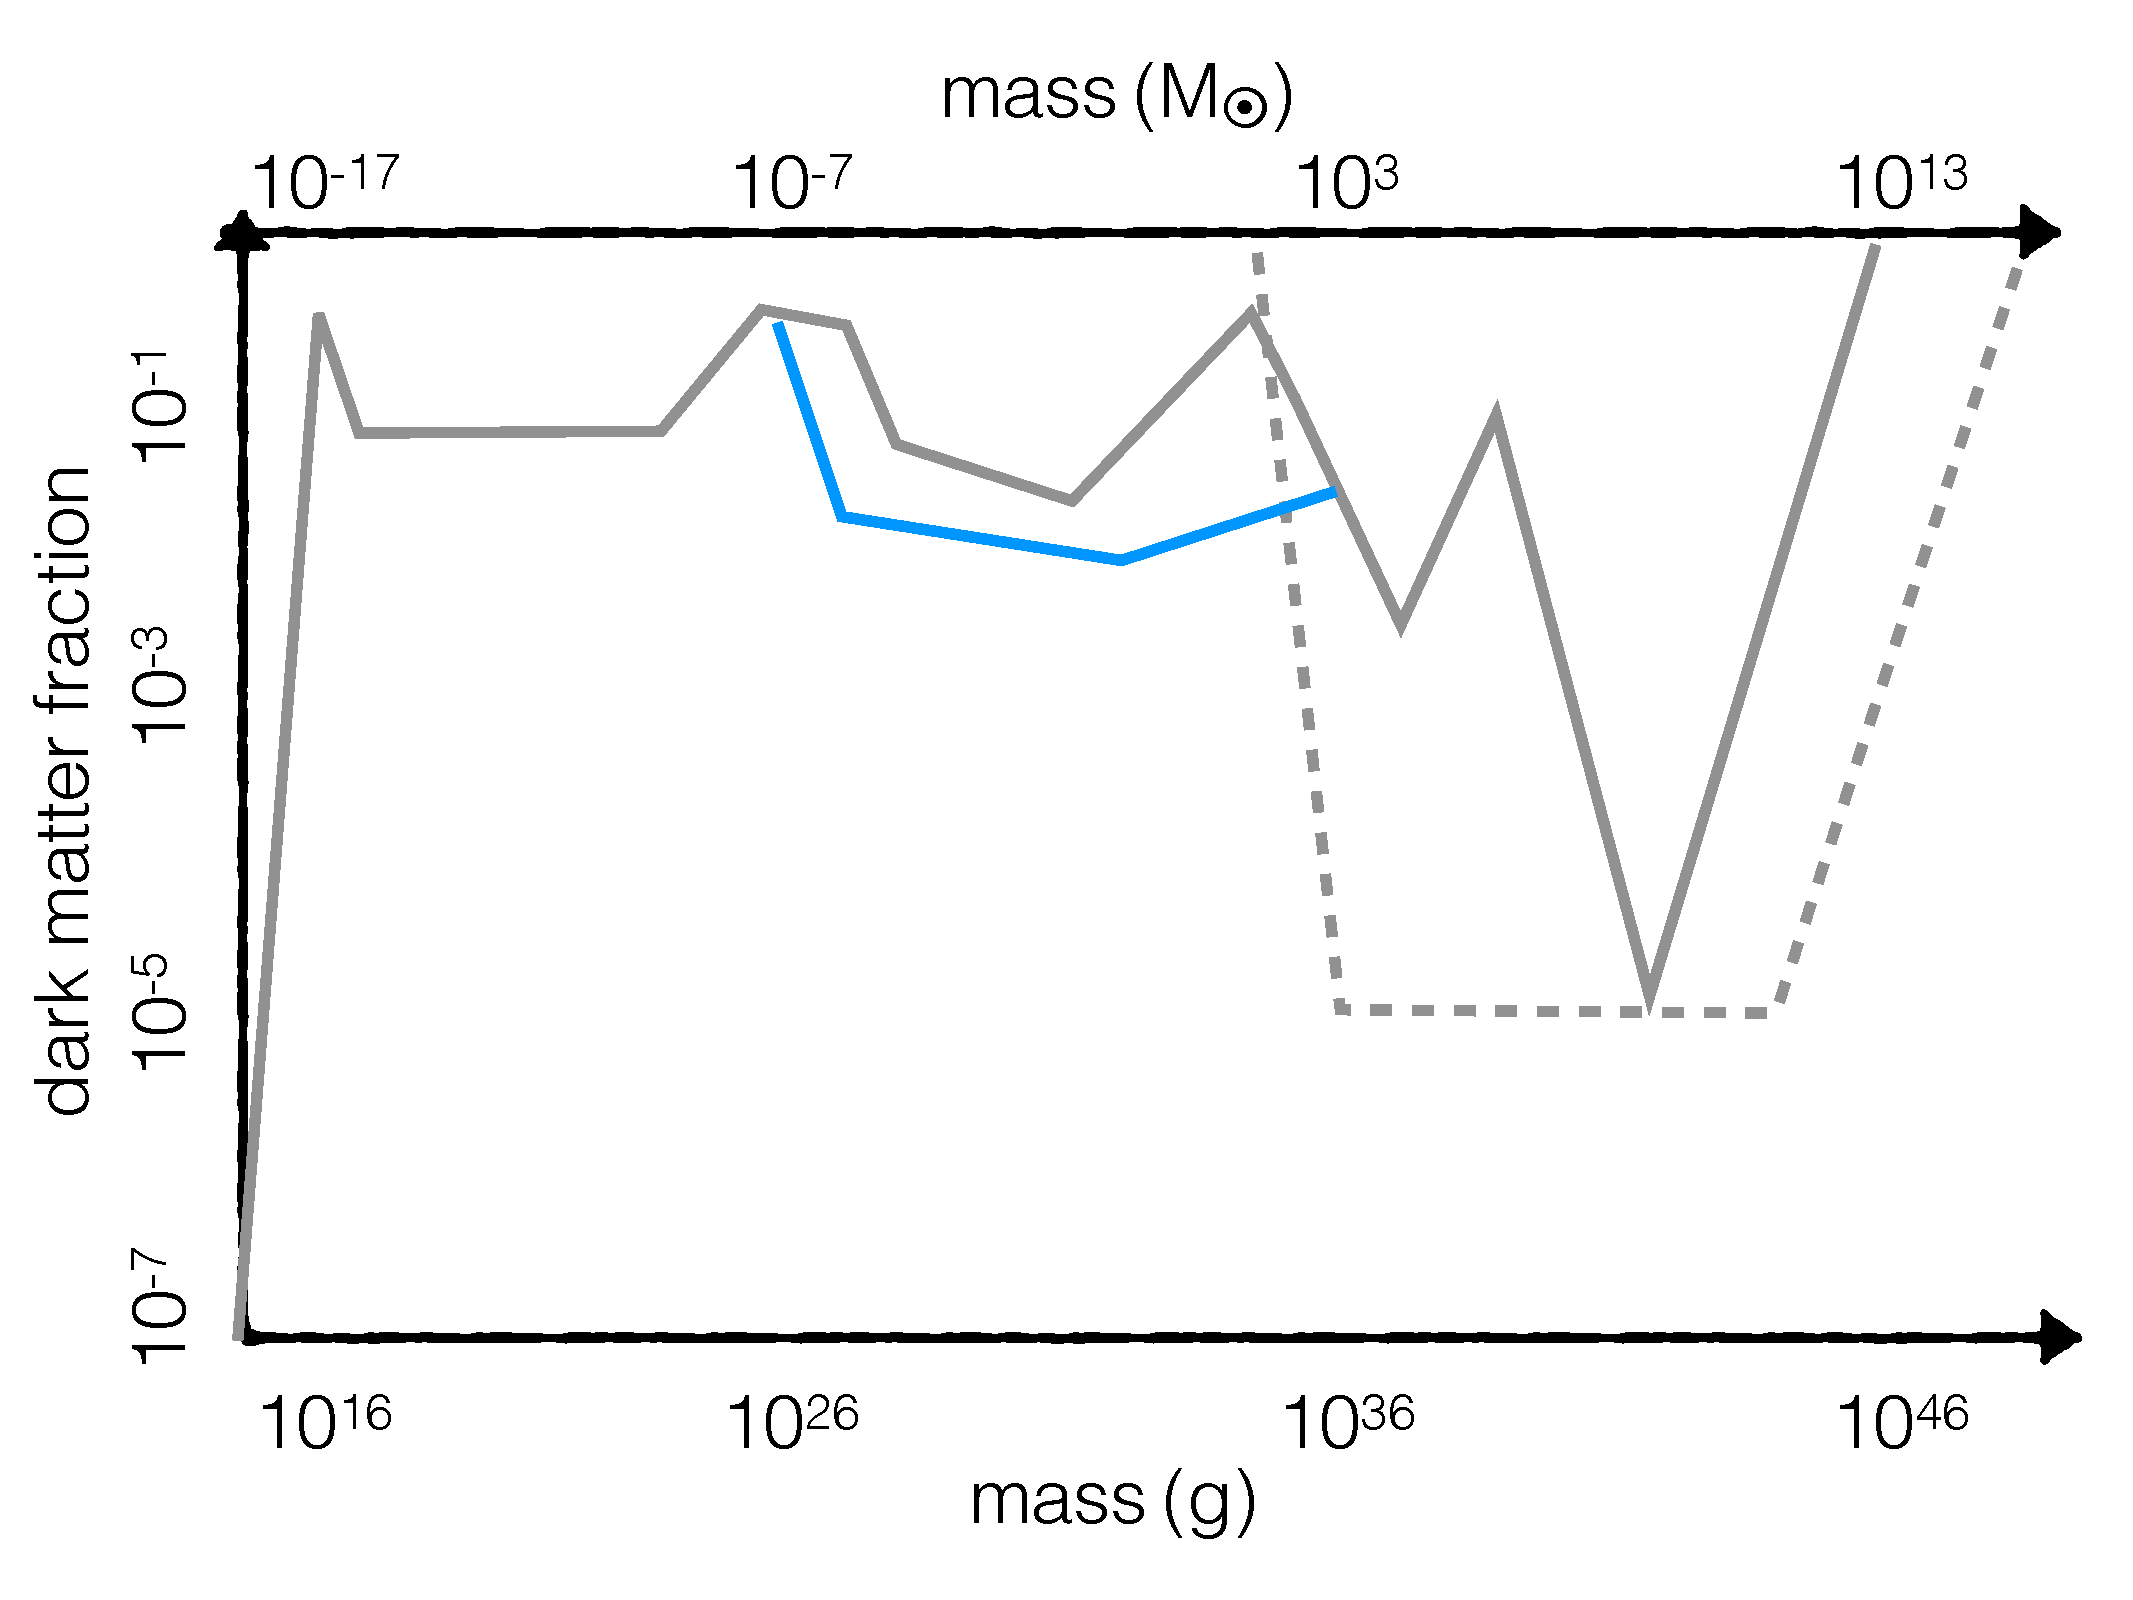
\includegraphics[width=0.6\columnwidth]{macho_cartoon.pdf}
%\caption{Fraction of dark matter that can be accounted for in compact objects.}
%\end{figure}

Dark matter in the form of compact objects, in particular black holes formed in the early universe, is one of the oldest and most venerable models of dark matter. Primordial black holes could originate from small-scale density fluctuations during the era of inflation. The same fluctuations that lay down the seeds of galaxies, if boosted on small scales, can lead to some small areas having a Schwarzchild mass within the horizon, which spontaneously collapse to form black holes. Because these black holes do not accrete or radiate strongly (at the time of formation there is no gas to form an accretion disc), they are a natural candidate for dark matter \citep{Carr:1974nx,Carr:2016drx}. 

Compact object dark matter is fundamentally different from particle models; black holes cannot be formed in an accelerator and can only be detected through their gravitational force. Current constraints suggest that primordial black holes do not make up all of the dark matter. However, primordial black holes are one possible source of the merging $30 M_\odot$ black holes recently detected by LIGO \citep{Bird:2016,Clesse:2016}. This possibility has rekindled interest in these objects, both as a source of dark matter and in their own right.

Limits on the abundance and mass range of primordial black holes are wholly observational. The black hole mass is set by the mass enclosed within the horizon at the time of black hole collapse and thus ranges between $10^{15}$ g ($10^{-18} M_\odot$), below which the black hole would evaporate, to $10^{42}$ g  ($10^9 M_\odot$), above which structure formation, big bang nucleosynthesis and the formation of the microwave background would be severely affected \citep{Sasaki:2018}. 
For $\sim $ stellar mass black holes, the gold standard technique for detecting compact objects is microlensing. Current microlensing constraints set limits on the black hole abundance at the level of $10\%$ for black holes $0.01 - 10 M_\odot$, see however \citep{Calcino:2018}. LSST will revolutionize the astrometric microlensing technique,  constraining the abundance of primordial black holes to a level of $10^{-4}$ of the dark matter over a wide range of masses (see Section \ref{sec:compact_object_abundance}).

As primordial black holes form directly from the primordial density fluctuations, measuring their abundance is a direct constraint on the amplitude of density fluctuations \citep{Clesse:2015}. Although these constraints are several orders of magnitude weaker than, for example, those from the microwave background, they probe small scales between $k = 10^{7} - 10^{19}$ $h$/Mpc, much smaller than those measured by other current and future probes \citep{Bringmann:2012}. Because these scales are highly non-linear in the late-time universe, there is no other possible constraint; the information present at early times has been washed away by gravitational evolution. Primordial black holes are thus a probe of primordial density fluctuations in a range that is inaccessible to other techniques\citep{Bellido:2017}.

These density fluctuations are imprinted at extremely high energies, beyond those currently accessible in terrestrial accelerators. 
At these high energies there are few theoretical constraints. Measurements of the primordial density fluctuations via the abundance of primordial black holes thus provide unique insights into physics at very high energies. \AHGP{NEED AN ENERGY SCALE}

%For example, the long lever of scales means that the constraints on simple scale-invariant inflation models expressed in terms of a scalar index, $n_s$ and a running, $\alpha_s$ can be competitive for some models. 

Furthermore, it may be possible for LSST to constrain the existence of ultra-compact mini-halos using correlated microlensing signals \citep{erickcek2011,li2012}. These objects arise from initial overdensities not large enough to collapse to a primordial black hole. These overdensities still collapse at high redshift to form low-mass halos. As these objects form early and have few mergers \citep{Bringmann:2011ut,Delos:2018}, they have a high concentration and a steeper internal density profile than the standard Navarro-Frenk-White shape, making them easier to detect via lensing and harder to disrupt than standard subhalos.

Current constraints on these objects are highly model-dependent; they come from assuming a WIMP dark matter annihilation cross-section and counting gamma-ray photons. LSST would place wholly new constraints on the existence of small halos from micro-lensing, and thus constrain the physics of the inflaton on scales of $k = 10 - 10^7 $ h/Mpc for the first time in a model-independent way.

%See Figure 6 of Bringmann 2012: \url{https://arxiv.org/abs/1110.2484}

%Sasaki 2018:
%\url{https://arxiv.org/abs/1801.05235}

%(probably belongs in the other section: observational constraints)
%Detection via microlensing is a gold standard in compact object observation as the only method capable of direct detection, setting limits on the mass of primordial black holes across a large range of mass scales. (reference to the signal part of the microlensing section). Other methods for detection of compact objects require indirect inference derived from models that make a large number of astrophysical assumptions. The only model required for measuring the mass of a compact object from the observation of microlensing is Einstein's theory of general relativity. LSST will provide excellent photometry of billions of stars over a timescale suitable for detecting primordial black holes up to thousands of solar masses. While systematics exist in photometric microlensing which must be addressed to make these measurements (reference to the systematics part of the microlensing section), current efforts are addressing these issues using reanalysis of the MACHO data. The Zwicky Transient Facility is also considered to a predecessor to LSST where additional microlensing surveys are prototyping the strategies of micrloensing detections on LSST. Complementary observations of astrometric microlensing using Keck AO, HST, and the next generation of large telescopes such as TMT and ELT will break the remaining degeneracies in these measurements and provide excellent mass measurements for compact object lenses.
